
%%%%%%%%%%%%%%%%%%%%%%%%%%%%%%%%%%%%%%%%%%%%%%%%%%%%%%%%%%%%%%%%%%%%%%%%%%%%%%%
%
% witseiepaper-2005.tex
%
%                       Ken Nixon (12 October 2005)
%
%                       Sample Paper for ELEN417/455 2005
%
%%%%%%%%%%%%%%%%%%%%%%%%%%%%%%%%%%%%%%%%%%%%%%%%%%%%%%%%%%%%%%%%%%%%%%%%%%%%%%%%

\documentclass[10pt,twocolumn]{witseiepaper}

%
% All KJN's macros and goodies (some shameless borrowing from SPL)
\usepackage{KJN}
\usepackage{hyperref}
\usepackage{xcolor}
\usepackage{caption}
\usepackage{subcaption}
%\usepackage{subfig}
\usepackage{pdfpages}
\usepackage{amsmath}
%
% PDF Info
%
\ifpdf
\pdfinfo{
/Title (INSTRUCTIONS AND STYLE GUIDELINES FOR THE PREPARATION OF FINAL YEAR LABORATORY PROJECT PAPERS : 2005 VERSION)
/Author (Ken J Nixon)
/CreationDate (D:200309251200)
/ModDate (D:200510121530)
/Subject (ELEN417/455 Paper Format, 2005)
/Keywords (ELEN417, ELEN455, paper, instructions, style guidelines, laboratory project)
}
\fi

%%%%%%%%%%%%%%%%%%%%%%%%%%%%%%%%%%%%%%%%%%%%%%%%%%%%%%%%%%%%%%%%%%%%%%%%%%%%%%%
\begin{document}
% HEARTBEAT SOUND SEGMENTATION AND CLASSIFICATION USING MULTI-DOMAIN FEATURES}

\title{\centering HEARTBEAT SOUND SEGMENTATION AND CLASSIFICATION USING MULTI-DOMAIN FEATURES}

\author{Elias Sepuru
\thanks{School of Electrical \& Information Engineering, University of the
Witwatersrand, Private Bag 3, 2050, Johannesburg, South Africa}
}


%%%%%%%%%%%%%%%%%%%%%%%%%%%%%%%%%%%%%%%%%%%%%%%%%%%%%%%%%%%%%%%%%%%%%%%%%%%%%%%
%
\abstract{For the majority, the only way to check-up for heart anomalies is to go to a medical practitioner for a check up and for most people especially in rural communities this hardly happens. This paper presents a method to create machine learning models that will enable first level screening of heart disease in smartphone and at hospitals. Two datasets from a smartphone and a digital stethoscope are used, yielding 24 features from four different domains.  The features are used to train an ANN, SVM and XGB. The models yield overall accuracies of 80\%, 78\% \& 79\% respectively. }

\keywords{MFCC, ANN, SVM, XGB, Wavelet}


\maketitle
\thispagestyle{empty}\pagestyle{empty}


%%%%%%%%%%%%%%%%%%%%%%%%%%%%%%%%%%%%%%%%%%%%%%%%%%%%%%%%%%%%%%%%%%%%%%%%%%%%%%%
%
\section{INTRODUCTION}
\label{intro}
As it stands, one of the most important, cost-effective and widely used techniques for one to get screened for cardiovascular diseases (CVDs) is through cardiac auscultation by a clinical physician \cite{32_montinari2019first}. For rural populations, screening for CVDs hardly occurs due to lack of clinical physicians and health care avoidance \cite{33,34}. World Health Organisation (WHO) reports CVDs as the leading cause of deaths globally, with an estimated 31\% of the deaths in 2016 caused by CVDs \cite{WHO}. Methods to detect early signs of CVDs could prove to be very helpful in lowering the mortality rate due to CVDs, especially in disadvantaged communities \cite{34}.

This paper presents a project, that aims create an application using machine learning techniques. The application will enable first level screening of CVDs for personal use by individuals on their smartphones and will aid clinical physicians with cardiac auscultation. To train the machine learning (ML) models, heartbeat sounds, in a form of a Phonocardiogram (PCG) signal, from two sources are used. The sources are a smartphone and a digital stethoscope. Prior training, the PCG signals are segmented and used to generate features to feed the ML models. A total of 24 features, including non-time-domain features, are extracted. The ML models (ANN, SVM \& XGB) trained on these features are then compared in their ability to diagnose CVDs.

%%%%%%%%%%%%%%%%%%%%%%%%%%%%%%%%%%%%%%%%%%%%%%%%%%%%%%%%%%%%%%%%%%%%%%%%%%%%%%%%%%%%%%%%%%%%%%%%%%%%%%%%%%%%%%%%%%%%%%%%%%%%%%%%%%%%

\section{BACKGROUND}
\label{back}
Through cardiac auscultation clinical physicians are able to tell whether an individual has CVDs or not. They use the heart's lub (S1) and dub (S2) sounds to help them identify irregularities in ones heartbeat sounds. S1 and S2 are known as the fundamental heart sounds (FHSs). The intervals between S1-S2 and S2-S1 are known as the systolic and diastolic periods respectively. For a relaxed heartbeat the diastolic period is larger than the systolic period \cite{orient2010sapira}. In a normal heartbeat sound, S1 is followed by S2 in a continuous cycle.

Abnormalities occur when there are irregularities in the cycle of S1 and S2, these irregularities are what makes CVDs. 

As mentioned in Section \ref{intro} , the heartbeat audio data is from two sources, a smartphone (Dataset A) and a digital stethoscope (Dataset B). Dataset A has four classes: Normal, Murmur, Extra Heart Sound (HS) and Artifact. Dataset B has has three classes: Normal, Murmur and Extrasystole. 

Murmurs are produced when there is a turbulent blood flow between either systolic or diastolic periods \cite{35}. The turbulence often cause a "whooshing" sound in between S1 and S2. Extra HS are produced when there is either an extra S2 or S1 after either S2 or S1 has occurred. This repeats regularly throughout the entire heart cycle in this manner: S1-S2-S2-S1 or S1-S1-S2-S1-S1. Extrasystole occur in a similar manner as Extra HS, but they do not occur regularly \cite{bentley}. See Appendix \ref{HS}, for a clearer explanation of the distinctions between the different classes and an explanation of the \hyperref[sec:arti]{Artifact} class.

\subsection{Project Framework}
\subsubsection{Project Specifications and Requirements}
\label{sec:req}
\textcolor{white}{Ke} %a leboga Ntate}\\
The ultimate aim of the project is create an application using ML techniques that will aid patients and clinical physicians in early detection of CVDs. The application is to accept raw audio data as input and return diagnosis results as an output.

This will be carried out using data from Dataset A and Dataset B. Dataset A is recorded by the general public using the iStethoscope Pro app on an iPhone, whilst Dataset B is recorded in a more professional manner by clinical physicians using a digital stethoscope. They both differ by two categories as mentioned in the opening paragraphs of Section \ref{back} and both have excessive background noise as they are recorded in real-life settings. 

Due to the excessive background noise, it is required that processing techniques capable of denoising the audio data be implemented before segmentation can occur. Following denoising, a method to locate S1 and S2 HSs as well as a method to segment the Normal PCGs from both datasets is required. After successful segmentation, it is required that features be generated from the results of segmenting the PCG signals. Lastly, it is required that ML models be built and trained using the generated features. 

\subsubsection{Assumptions}
\textcolor{white}{Ke a leboga Jeso}\\
The project is to be conducted under the following assumptions:
\begin{itemize}
    \item The audio data range will be 30 seconds or less.
    \item Dataset A has only four classes ( Normal, Murmur, Extra HS and Artifact). Dataset B has only three classes ( Normal, Murmur \& Extrasystole)
    \item Both datasets have integrity and are correctly labelled.
\end{itemize}

\subsubsection{Constraints}
\label{sec:constraints}
\textcolor{white}{O re swarele...}\\
The following are the constraints imposed on the project:
\begin{itemize}
    \item Segmentation is based only on S1 and S2 sounds.
    \item Only the dataset from reference \cite{bentley} is to be used due to ethics clearance.
    \item Only the Normal audio data will be used as a basis for the location of S1 and S2 and as a basis for segmentation.
    \item The audio data is only available in \texttt{.wav} and \texttt{.aif} formats.
\end{itemize}

\subsubsection{Success Criteria}
\textcolor{white}{O re swarele...}\\
The project is deemed successful if all requirements in Section \ref{sec:req} have been met, whilst adhering to the set constraints in section \ref{sec:constraints}. Existing solutions
have an accuracy of up to 77\% for classifying Normals of Dataset B and an accuracy of up to 46\%
for Normals of Dataset A. With that said an accuracy of 77\% or higher in classifying Normals of Dataset B and
an accuracy of 46\% or higher in classifying Normals of Dataset A would be highly desirable.

\subsection{Related Work}
\label{sec:lit}
Despite the medical significance of using ML techniques to detect for heart sounds (HSs) anomalies, this application of ML is relatively unexplored \cite{bentley}. There also exist a few studies that have done work in classifying various heartbeat sounds using these techniques \cite{26}. Of a few that exist majority of them use PCG signals \cite{22,3} whilst others use Electrocardiograms (ECG) signals \cite{5}. 

Before classification can occur, the HSs have to first be preprocessed and segmented. Liang \textit{et al} \cite{6} dominate in a lot of work \cite{22,15} with their method of preprocessing and segmenting HSs.  

The features extracted from segmentation of HSs are usually time-domain based. Strunic \textit{et al} \cite{3} detects and classifies simulated murmurs \& normal HSs using similar preprocessing and segmentation techniques to \cite{6}. He trains a 3 hidden layer, 25 input and 1 output Artificial Neural Network (ANN) with simulated HSs. The ANN classifier achieves an accuracy of $85\pm7.4\%$ when tested with simulated HSs, however when tested with real-life HSs the accuracy drops to $48.7\pm12.7\%$. Unlike Strunic, Gomes \textit{et al} \cite{gomes2012classifying} train their ML models with real-life HSs having background noise. They extract time-domain features as well, using the standard deviation and mean of the systolic and diastolic periods intervals of the HSs. They achieve the highest accuracy of 72\% \& 70\% in classifying Normal HSs using the J48 Decision Tree and Multilayer Perceptron (MLP) respectively.

Instead of using time-domain features, Teo \textit{et al} \cite{17} segment HSs on the basis of S1, S2, systolic and diastolic periods. They take the Fast Fourier Transform (FFT) and Power Spectrum of each of the four segments and use them to train their Neural Network (NN).The NN achieves a total diagnosing accuracy of  77\%. 

Zhang \textit{et al} \cite{16} notice that using time or frequency domain features independently causes a loss in important pathological information. This leads to Tang \textit{et al} \cite{22} taking it one step further by combining a set of features from the time-domain, frequency-domain, cepstrum \& energy amongst others. With the same dataset as \cite{17}, they achieve an overall accuracy of 88\% using a Support Vector Machine (SVM) classifier.

%%%%%%%%%%%%%%%%%%%%%%%%%%%%%%%%%%%%%%%%%%%%%%%%%%%%%%%%%%%%%%%%%%%%%%%%%%%%%%%%%%%%%%%%%%%%%%%%%%%%%%%%%%%%%%%%%%%%%%%%%%%%%%%%%%%%
\section{SYSTEM OVERVIEW}
The main framework of this project is illustrated in figure \ref{fig:frame}. The framework presents the ML models development of the project. On signal processing, this paper mainly focuses on the FFT, MFCC \& Wavelet. Preprocessing and Segmentation are covered in more detail in \cite{love}. Feature Generation, ML model training and ML model testing are also covered in detail in this paper.

\begin{figure}[h!]
    \centering
    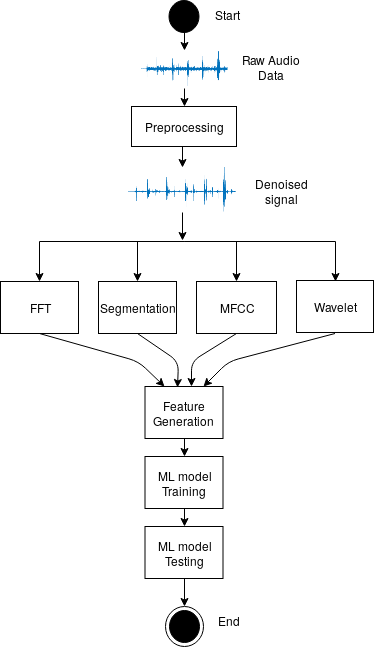
\includegraphics[scale=0.5]{./framework2.png}
    \caption{Project framework}
    \label{fig:frame}
\end{figure}

From figure \ref{fig:frame}, the raw audio data is read from the two datasets in either formats mentioned earlier. As the audio data contains extensive background noise, they first pass through preprocessing, where they are denoised. After denoising, the PCG signals go through four parallel stages for further signal processing. The four parallel stages condition the PCG signals for feature extraction in their respective domains. Once features from all four domains are generated, the development of ML models begin. The models are trained of the features. After training the models, testing begins.
%%%%%%%%%%%%%%%%%%%%%%%%%%%%%%%%%%%%%%%%%%%%%%%%%%%%%%%%%%%%%%%%%%%%%%%%%%%%%%%%%%%%%%%%%%%%%%%%%%%%%%%%%%%%%%%%%%%%%%%%%%%%%%%%%%%%

\section{IMPLEMENTATION}
\subsection{Dataset}
As mentioned in Section \ref{back}, there are two datasets that are used to train \& test the ML models. Dataset A is collected from the general public and is recorded using an iPhone application, iStethoscope pro. The dataset has four classes and a total of 124 samples of a sample rate 44100 Hz. Dataset B on the other hand, is recorded using a digital stethoscope, DigiScope. The dataset is collected by clinical physicians in hospitals at a sample rate of 4000 Hz. The total count of the samples in the dataset amounts to 312 with three classes \cite{bentley}. Figure \ref{fig:dist} illustrates the distribution of both the datasets on the same axis.

\begin{figure}[h!]
    \centering
    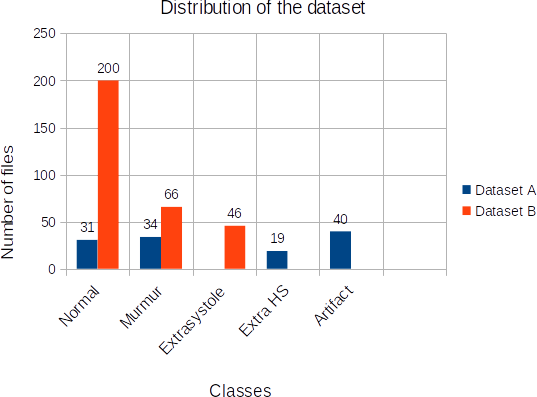
\includegraphics[scale=0.45]{./distribution.png}
    \caption{Distribution of the datasets}
    \label{fig:dist}
\end{figure}

From figure \ref{fig:dist}, it can be seen that Dataset A's data is somewhat evenly distributed whilst Dataset B's data is not.

\subsection{Preprocessing \& Segmentation}
\label{sec:preseg}
The preprocessing phase is where the HSs are denoised as seen in figure \ref{fig:frame}. In this phase the PCG signals from both datasets are downsampled to a common sampling frequency of 2000 Hz. The signals are then normalised. After normalisation the signals go through a range of denoising techniques, including bandpass filtering and wavelet denoising. 

After preprocessing, the segmentation phase begins. In this phase, S1 and S2 are located on the preprocessed HSs. The HSs are then segmented on the basis of the located FHSs. Figure \ref{fig:preseg} in Appendix \ref{app:preseg} summarises the Preprocessing and Segmentation phase, for a clearer and concise explanation of this phase see \cite{love}.

\subsection{Feature Extraction}
\label{sec:feat}
As stated in Section \ref{sec:lit}, multi-domain features make up for a more accurate representation of the different classes of HSs \cite{22}. In this project features from the time, frequency, cepstrum \& wavelet domain are engineered for ML. A total count of 24 features are extracted.

\subsubsection{Time Domain Features}
\textcolor{white}{Ke na le modisa...}\\
Time domain features are features extracted from the results of \hyperref[sec:preseg]{segmentation}. Given the location of S1 \& S2, the diastolic and systolic intervals of the HSs are determined. Features are then taken from computing the standard deviation \& mean of the systolic and diastolic intervals, other features are taken from relating the number of peaks and the file length. A total of 10 features are extracted from the time-domain, making up the majority of the extracted features. Table \ref{tab:tfeat} in Appendix \ref{app:features} elaborates more on the time-domain features extracted.

The motivation for computing the standard deviation and mean of the HSs' systolic \& diastolic intervals is both from literature \cite{gomes2012classifying,bentley} and observation. It was observed that in most cases Normal HSs have a \hyperref[t:s1]{\texttt{stdS1}} \& \hyperref[t:s2]{\texttt{stdS2}} of less than or equal to a 100. From conducting the project it was also observed that Extra HS and Extrasystole HSs have more peaks per file length hence the motivation behind \hyperref[t:pr]{\texttt{prRatio}} \& \hyperref[t:pc]{\texttt{pcRatio}}.

\subsubsection{Wavelet Features}
\textcolor{white}{Ke tlabe ke hlokang...}\\
In preprocessing, there is a part where the wavelet transform is used to denoise the PCG signals, see figure \ref{fig:preseg} in Appendix \ref{app:preseg} and \cite{love}. The denoising is carried out using a fifth level $7^{th}$ order Daubechies (db7) Discrete Wavelet Transform (DWT). 

To denoise, the DWT decomposes and reconstructs the original signal using wavelet approximations, leaving out noisy components of the signal. The reconstruction often under-approximate murmurs \cite{10}. This leads to an important features in classifying the Murmur class. The feature, \texttt{rebuildError}, as the name suggests is constructed by taking the average of the difference between the original PCG signal just before wavelet denoising and the PCG signal after wavelet denoising. Figure \ref{fig:dbb} and figure \ref{fig:dba} illustrate the normalised \texttt{rebuildError} of PCG signals in Dataset A and Dataset B respectively.

\begin{figure}[h!]
    \centering
    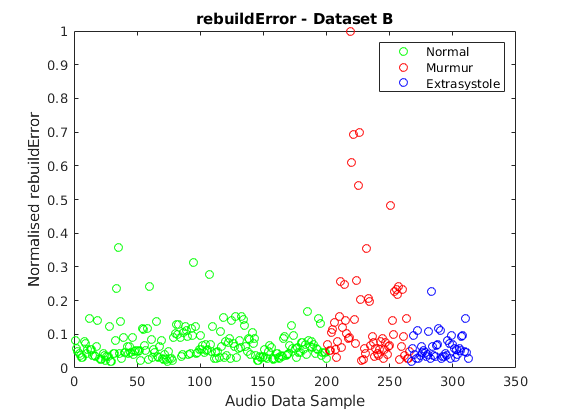
\includegraphics[scale=0.45]{./rebuildError_B.png}
    \caption{\texttt{rebuildError} amongst the different classes in Dataset B}
    \label{fig:dbb}
\end{figure}

\begin{figure}[h!]
    \centering
    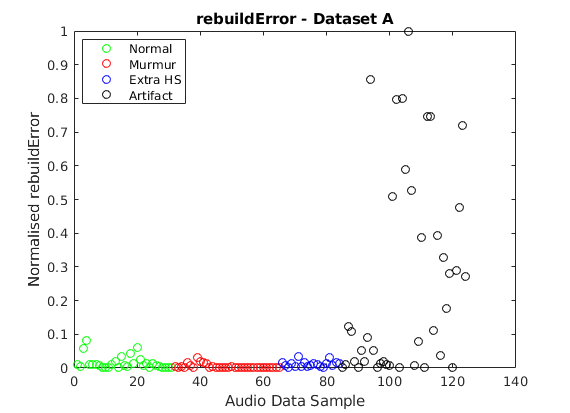
\includegraphics[scale=0.45]{./rebuildError_A.png}
    \caption{\texttt{rebuildError} amongst the different classes in Dataset A}
    \label{fig:dba}
\end{figure}

From figure \ref{fig:dbb} it is clear that in Dataset B, the Murmur class has the largest \texttt{rebuildError} as compared to the other classes. Figure \ref{fig:dba} on the other hand shows the Artifact class in Dataset A having the highest \texttt{rebuildError}. The other wavelet features are computed by taking the mean and standard deviation of the approximation of a $6^{th}$ level db6 DWT of the preprocessed PCG signals. See table \ref{tab:wav} in Appendix \ref{app:features}. Features from the wavelets make up only 3 out of the 24 total features.


\subsubsection{Frequency Domain Features}
\textcolor{white}{Ke ea ipit}\\
Features in the frequency domain are computed by taking the FFT of the PCG signals. Through experimentation, it was discovered that murmurs tend to have distinct peaks between 180 Hz \& 190 Hz bands of their analytic envelope of their FFT. The analytic envelope computed using the FFT of a PCG signal will be termed FFTSHA for the rest of this paper. Steps followed on how the FFTSHA of a PCG signal is computed are explained concisely in Appendix \ref{app:features} Section \ref{sec:fftsha}. 

Figure \ref{fig:n180} and figure \ref{fig:m180} show the difference in the FFTSHA of PCG signals in the Normal class and Murmur class respectively.

\begin{figure}[h!]
    \centering
    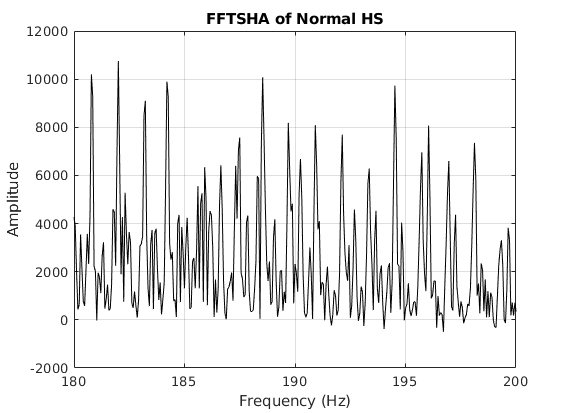
\includegraphics[scale=0.45]{./fftsha_n.png}
    \caption{FFTSHA of a Normal PCG signal at [180 190] Hz band.}
    \label{fig:n180}
\end{figure}

\begin{figure}[h!]
    \centering
    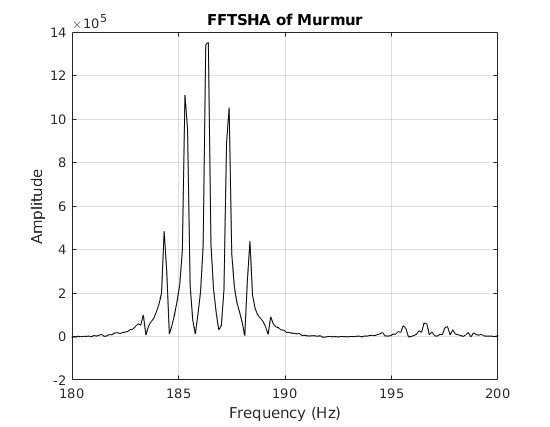
\includegraphics[scale=0.45]{./fftsha_m.png}
    \caption{FFTSHA of a Murmur PCG signal at [180 190] Hz band.}
    \label{fig:m180}
\end{figure}

Peaks are identified in a similar as \cite{love} from the [180 190] Hz as seen in figure \ref{fig:n180} \& figure \ref{fig:m180}. From the identified peaks features are generated. Table  \ref{tab:freq} in Appendix \ref{app:features} elaborates more on the features extracted. Features from the frequency-domain make up 5 out of the 24 total number of features.

\subsubsection{Cepstrum Features}
\textcolor{white}{Modimo yo a phelang...}\\
The cepstrum is defined as the inverse Fourier transform (IFT) of the log-magnitude of the Fourier Transform (FT). Mel-Frequency Cepstrum Coefficients (MFCC) are an advancement of the cepstrum. MFCC approximates the human ear perception of distance in frequency \cite{24}. MFCC are commonly used for voice recognition.

To extract cepstrum features, 12 MFCC coefficients are extracted from each PCG signal. After extraction of the coefficient vectors, Principal Component Analysis (PCA)  is performed on the vectors. PCA pushes all the important features of the 12 coefficient vectors into the first couple of vectors. From applying PCA to the MFCC feature coefficients, features are extracted by computing the mean and standard deviation PCA vectors. Table \ref{tab:cep} in Appendix \ref{app:features} further elaborates on the features. A total of 6 out 24 features are extracted from the cepstrum domain.

\subsection{Classification}
In the classification phase, ML models are trained, validated and tested with features extracted in Section \ref{sec:feat}. Three ML models, ANN, SVM \& XGBoost (XGB) are used to classify the HSs. After numerous iterations of the three models with both datasets, it was discovered that Dataset A is best suited with 21 features. Dropping \texttt{stdWavelet, meanWavelet \& pcRatio} from Dataset A.

\subsubsection{Artificial Neural Network}
\textcolor{white}{O nkisa botaleng..}\\
ANNs are considered to be good algorithms for pattern detection \cite{3}. The ANN designed to train on features from Dataset B has 24 input neurons, 1 hidden layer and 3 output neurons. The ANN designed for Dataset A is similar to the one for Dataset B, the only difference is in the input and output neurons. To avoid overfitting for Datset A a dropout of 0.25 is used. Both Datasets are split on 6:2:2 for training, validation \& testing respectively. After numerous iterations, it was discovered that 1 hidden layer is sufficient for both the models.

\subsubsection{Support Vector Machines}
\textcolor{white}{Meetseng a mphedisang..}\\
SVMs have seen a rise in popularity in the past years \cite{5}. This is due to their ability to separate different classes by developing an optimal hyperplane between them \cite{22}. To train the model the dataset is split on 8:2. Before training or testing can occur, parameter optimisation is performed with \texttt{GridSearchCV} to see which parameters are optimal to train the model. After getting optimal parameters the model is trained and tested.

\subsubsection{XGBoost}
\textcolor{white}{O nkalosa dinokoaneng..}\\
The XGBoost is a scalable ML Model and gives a state of the art results in a wide range of problems. It also has a reputation of winning Data Science and ML challenges. Of all the challenges hosted by Kaggle, teams having an XGBoost model have won the most \cite{45}. To train, the data is split on 8:2. Before training commences, parameter optimisation is performed. After finding the optimum parameters the model is redesigned, trained and tested.

\section{RESULTS}
The models are evaluated using three metrics from \texttt{sklearn} library in Python. The methods are the confusion matrix, the accuracy score and classification report. On the ANN the score is replaced by the training and testing accuracy. Figure \ref{fig:anna} and figure \ref{fig:annb} in Appendix \ref{app:res} illustrate the testing and training accuracy for Dataset A and Dataset B respectively.

Table \ref{datasetA} and Table \ref{datasetB} show the precision of all the classes and the overall performance of for each model for both Dataset A and Dataset B. The models' performance are compared with the one in literature \cite{bentley}.
\begin{table}[h!]
\centering
\caption{Classification Performance Dataset-A}
\label{datasetA}
\begin{tabular}{|c|c|c|c|c|}
\hline
\textbf{\begin{tabular}[c]{@{}c@{}}Class\\ (A)\end{tabular}} & \textbf{\begin{tabular}[c]{@{}c@{}}ANN\\ (\%)\end{tabular}} & \textbf{\begin{tabular}[c]{@{}c@{}}SVM\\ (\%)\end{tabular}} & \textbf{\begin{tabular}[c]{@{}c@{}}XGB\\ (\%)\end{tabular}} & \textbf{\begin{tabular}[c]{@{}c@{}}Liter-\\ ature(\%)\end{tabular}} \\ \hline
Normal & 27 & 80 & 71 & 45 \\ \hline
Murmur & 88 & 78 & 86 & 31 \\ \hline
ExtraHS & 67 & 25 & 57 & 11 \\ \hline
Artifact & 100 & 57 & 50 & 58 \\ \hline
\begin{tabular}[c]{@{}c@{}}Overall\\ Accuracy\end{tabular} & \textbf{81} & \textbf{64} & \textbf{68} & \textbf{46} \\ \hline
\end{tabular}
\end{table}

\begin{table}[h!]
\centering
\caption{Classification Performance Dataset-B}
\label{datasetB}
\begin{tabular}{|c|c|c|c|c|}
\hline
\textbf{\begin{tabular}[c]{@{}c@{}}Class\\ (B)\end{tabular}} & \textbf{\begin{tabular}[c]{@{}c@{}}ANN\\ (\%)\end{tabular}} & \textbf{\begin{tabular}[c]{@{}c@{}}SVM\\ (\%)\end{tabular}} & \textbf{\begin{tabular}[c]{@{}c@{}}XGB\\ (\%)\end{tabular}} & \textbf{\begin{tabular}[c]{@{}c@{}}Liter-\\ ature(\%)\end{tabular}} \\ \hline
Normal & 80 & 77 & 89 & 78 \\ \hline
Murmur & 90 & 87 & 75 & 37 \\ \hline
Extrasys & 15 & 0 & 17 & 17 \\ \hline
\begin{tabular}[c]{@{}c@{}}Overall\\ Accuracy\end{tabular} & \textbf{80} & \textbf{78} & \textbf{79} & \textbf{77} \\ \hline
\end{tabular}
\end{table}

\section{CRITICAL ANALYSIS}

From the ANN epoch graphs illustrated by figure \ref{fig:anna} \& figure \ref{fig:annb} in Appendix \ref{app:res} for Dataset A and Dataset B respectively, there is no sign of overfitting. This suggests that both the ANN models are not bias.

Comparing the models' performances in both datasets it can be seen that the models work better on Dataset B. This is because Dataset B's HSs were recorded by professionals in a professional setting compared to Dataset A which was recorded by the general public using a smartphone i.e Dataset A is more noisy. Another role player is sample size, Dataset A has a lower sample size compared to Dataset B. ML is all about the more data one has, the better the model. 

The models performance on Dataset A is somewhat distributed amongst the different classes whilst on Dataset B the performance is skewed with ranges of up to 87. This because as seen from figure \ref{fig:dist}, Dataset A samples are distributed whilst Dataset B's samples are skewed. This means that the models learn more about Normals \& Murmur HSs compared to Extrasystole HSs.

In general all the models performed better than what is in literature.  With ANN almost tripling the precision of Murmurs in literature. However the models still struggle with Extrasystole HSs due to the size of the samples and also due to the fact that they are similar to Normal HSs. The confusion matrix in Appendix \ref{app:res} show that Extrasystole HSs are often mistaken for Normal HSs.

\section{FUTURE RECOMMENDATIONS}
For future work algorithms that can differentiate between Extrasystole HSs and Normal HSs needs to be implemented, techniques such as the ones in \cite{17} could be used. A larger and evenly distributed dataset can also greatly improve the ML model's accuracy. 

\section{CONCLUSION}
A method to create models that will enable first level screening of CVDs is successfully implemented. Two datasets from a digital stethoscope and a smartphone are used, from the two datasets 24 features from the time, frequency, cepstrum \& wavelet domain are extracted. The features are used to train ANN, SVM \& XGB. The precision results  of 80\%, 77\% \& 89\% meet the success criteria set for Normals of Dataset B. The shortcomings of the models include not being able to successfully identify Extrasystole HSs, more work is required in this regard. 

%%%%%%%%%%%%%%%%%%%%%%%%%%%%%%%%%%%%%%%%%%%%%%%%%%%%%%%%%%%%%%%%%%%%%%%%%%%%%%%


%%%%%%%%%%%%%%%%%%%%%%%%%%%%%%%%%%%%%%%%%%%%%%%%%%%%%%%%%%%%%%%%%%%%%%%%%%%%%%%
%

%\nocite{*}
\bibliographystyle{witseie}
\bibliography{sample}

%{\tiny \vfill \hfill \today \hspace{5mm} witseie-paper-2003.\TeX}



%%%%%%%%%%%%%%%%%%%%%%%%%%%%%%%%%%%%%%%%%%%%%%%%%%%%%%%%%%%%%%%%%%%%%%%%%%%%%%%%%%%%%%%%%%%%%%%%%%APPENDIX%%%%%%%%%%%%%%%%%%%%%%%%%%%%%%%%%%%%%%%%%%%%%%%%%%%%%%%%%%%%%%%%%%%%%%%%%%%%%%%%%%%%%%%%%%%%%%%%%%%%%%%%%%%%%%%%%%%%%%%%%%%%%%%%%%%%%%%%%%%%%%%%%%%%%%%%%%%%%%


\newpage
\onecolumn
\appendices

%%%%%%%%%%%%%%Group Reflection%%%%%%%%%%%%%%%%%%%%%%
\section{Reflection on Group Work}

\subsection{\textbf{Introduction}}
In this document I will be discussing the division of work amongst the members of the group and also my personal reflection on my experience of working in a group.

\subsection{\textbf{Work Division}}
During the first week, me and my partner, Boikanyo Radiokana both started off with reading papers together because we did not fully understand what what required of us. At first we thought the final project required each member to write about the whole project, hence we wanted equal exposure to all sections in the project. When we learned that for the final project, each member should focus on the section they mostly did, we divided work equally amongst ourselves. The table below shows the work division amongst us:

\begin{table}[h!]
\centering
\caption{Work Division}
\label{undefined}
\begin{tabular}{|l|l|}
\hline
\textbf{Task} & \textbf{Team Member} \\ \hline
Preprocessing & Boikanyo \\ \hline
Segmentation & Boikanyo \\ \hline
Feature Extraction & Elias \\ \hline
Classification & Elias \\ \hline
GUI Front-end & Boikanyo \\ \hline
GUI Back-end & Elias \\ \hline
GUI Integration & Boikanyo and Elias \\ \hline
Project Poster & Boikanyo and Elias \\ \hline
\end{tabular}
\end{table}

\subsection{\textbf{Lessons Learned}}
Throughout the project life cycle I learned that sometimes no matter how much you try, 
things will not always be the way you expect them to be. I have learnt the art of letting go, not everything will be 100\% accurate.

\subsection{\textbf{Personal Reflection}}
This project has taught me to appreciate the input of my others in a group. I got to experience shared responsibilities. I didn't have to worry about anything because my partner always delivered on her part. I enjoyed working in a group and learned a thing or two about myself. I am pleased with how everything turned out.

\subsection{\textbf{Conclusion}}
Overall the project was a success and I enjoyed working in a group. Tasks were evenly allocated to team members who equally delivered.
%%%%%%%%%%%%%%Lab specifications%%%%%%%%%%%%%%%%%%%%%%
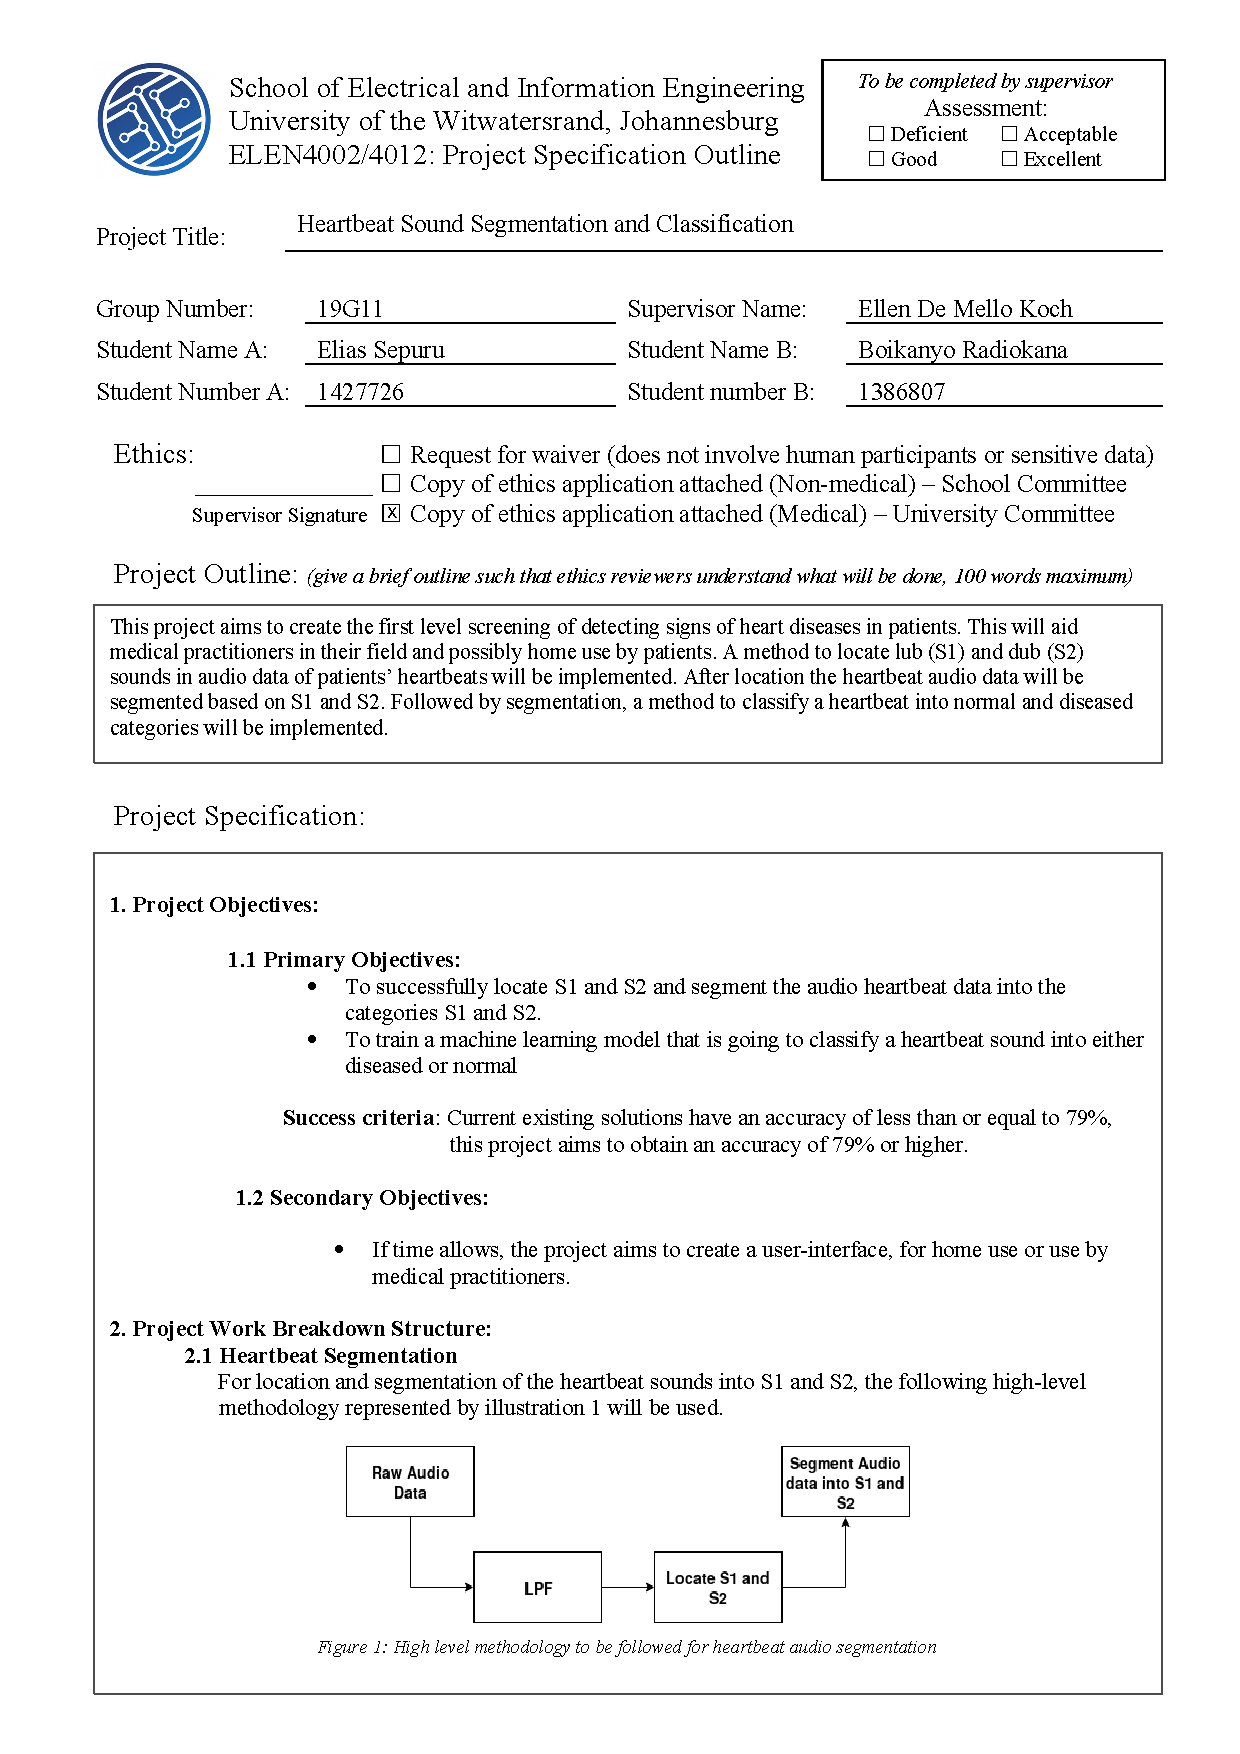
\includepdf[scale=0.94,pages=1,pagecommand={\section{Project Specification}\thispagestyle{empty}},fitpaper=true]{labspecs.pdf}
\includepdf[scale=0.94,pages=2,pagecommand={\thispagestyle{empty}},fitpaper=true]{labspecs.pdf}

%%%%%%%%%%%%%%Project Plan%%%%%%%%%%%%%%%%%%%%%%
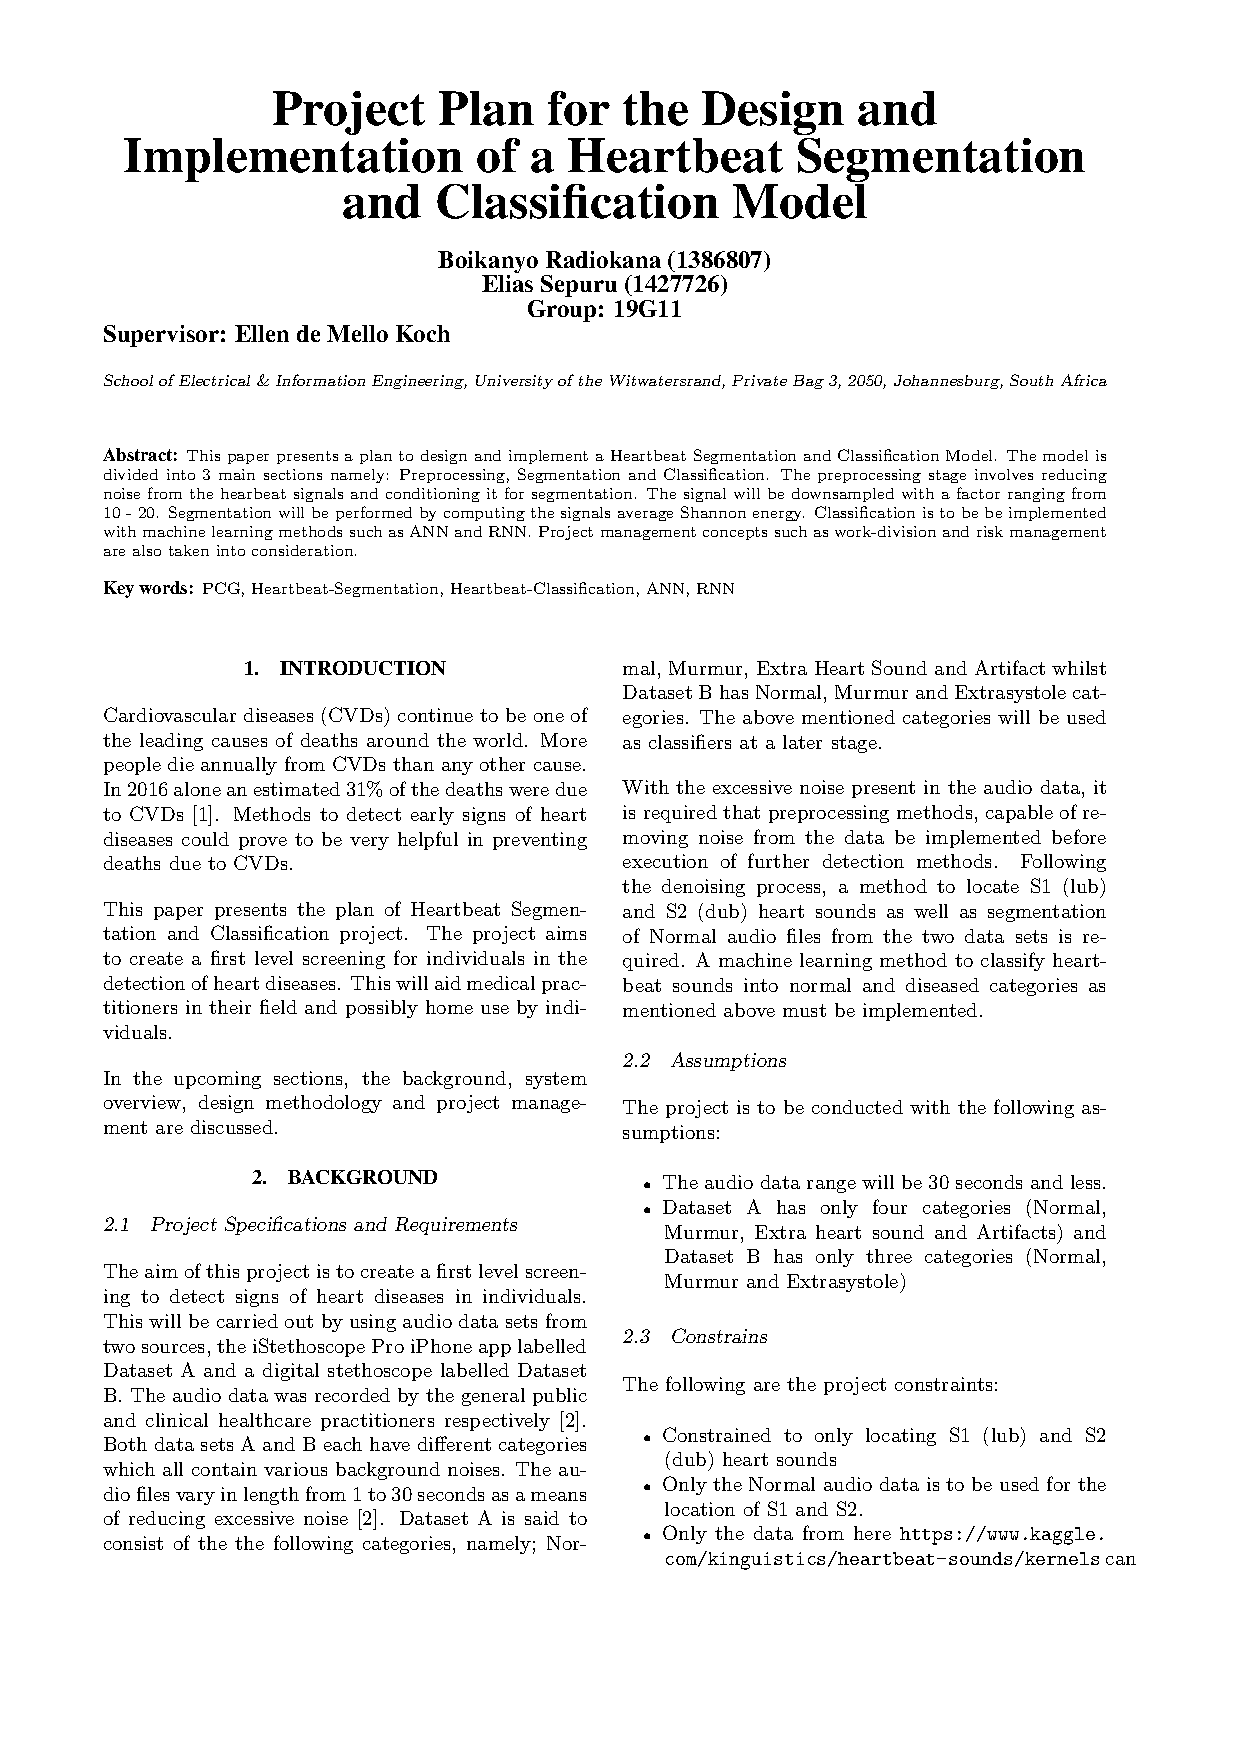
\includepdf[scale=0.94,pages=1,pagecommand={\section{Project Plan}\thispagestyle{empty}},fitpaper=true]{projectPlan.pdf}
\includepdf[scale=0.94,pages=2-6,pagecommand={\thispagestyle{empty}},fitpaper=true]{projectPlan.pdf}


%%%%%%%%%%%%%%Clearance Certificate%%%%%%%%%%%%%%%%%%%%%%
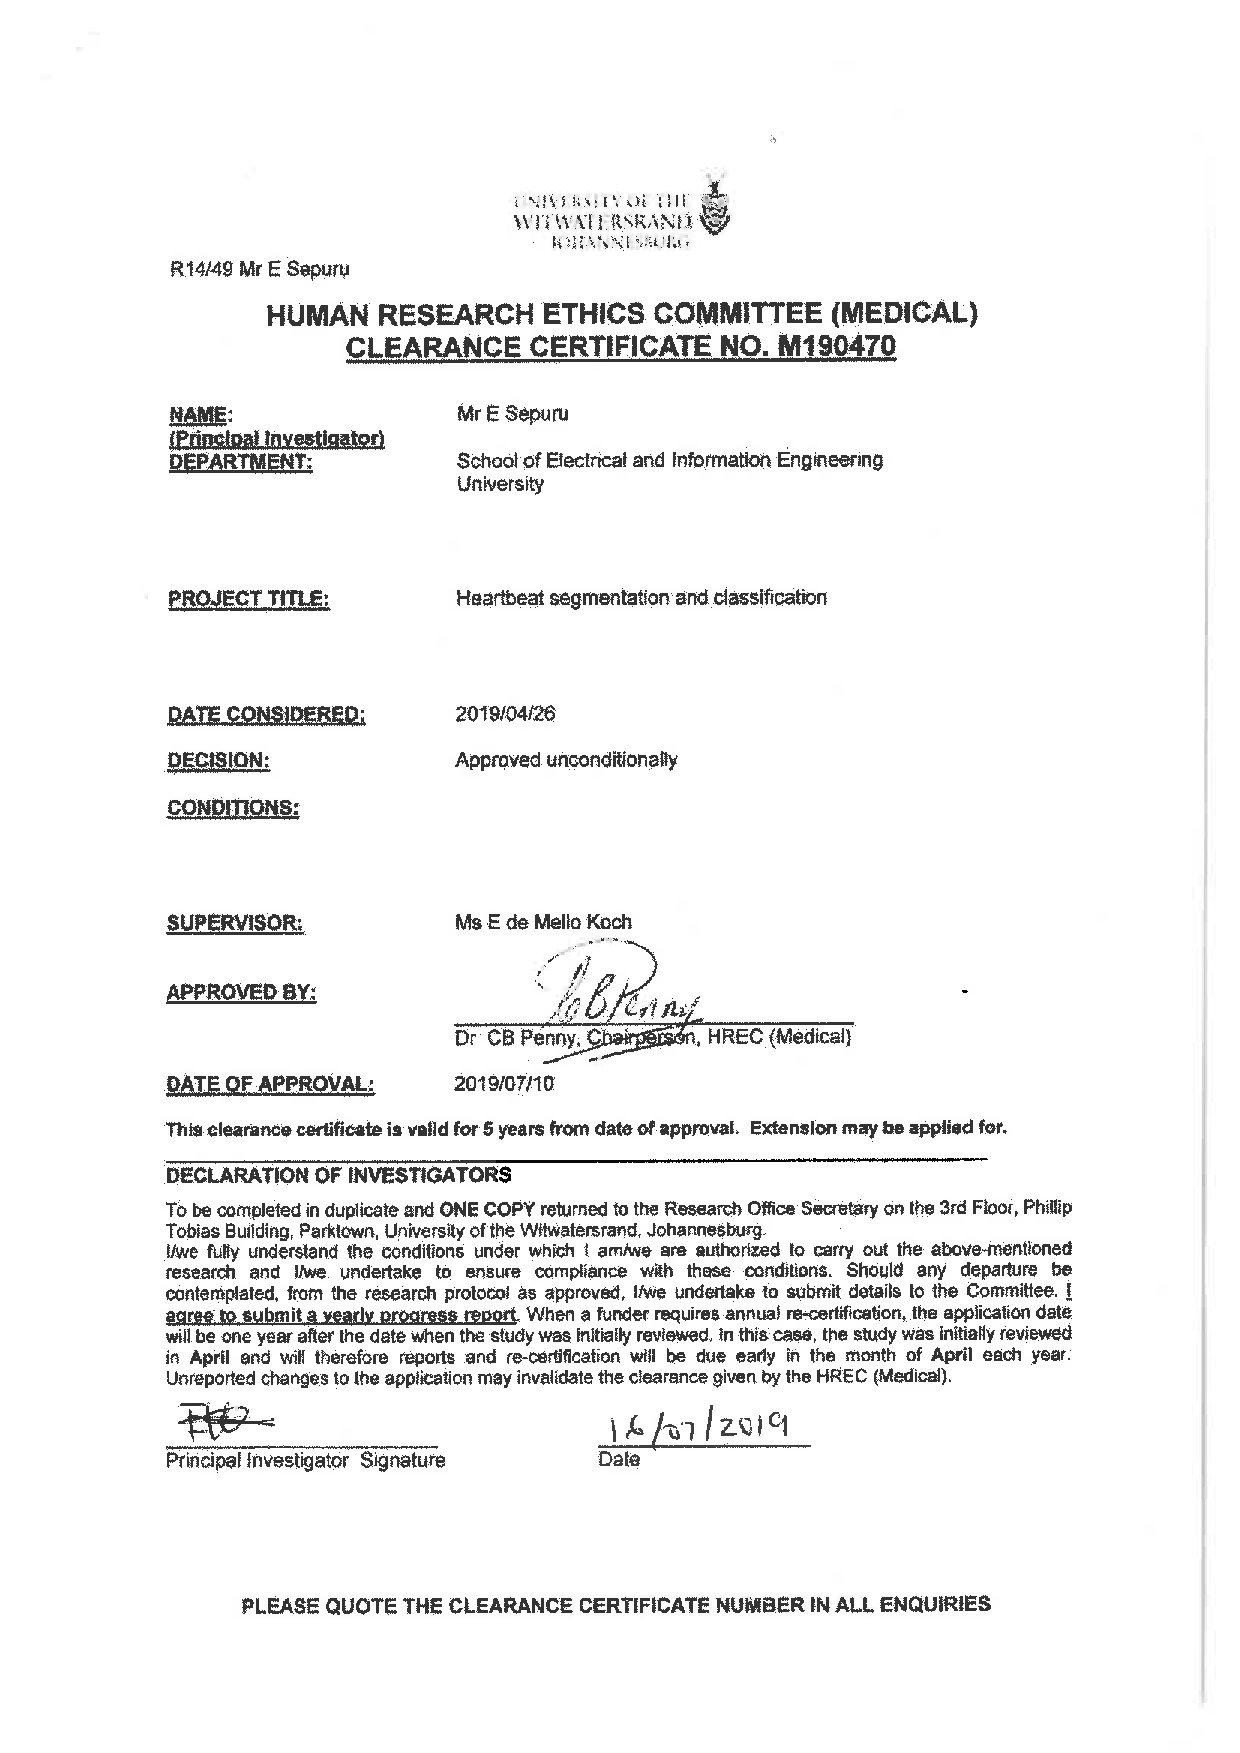
\includepdf[scale=0.94,pages=1,pagecommand={\section{ETHICS CLEARANCE CERTIFICATE}\thispagestyle{empty}},fitpaper=true]{clearanceCertificate.pdf}

%%%%%%%%%%%%%%%%%%%%%%%%
\twocolumn
\section{Heart Sound Classes}
\label{HS}

\subsection*{The Normal Class}
The Normal class consists of normal, healthy and regular HS. A Normal HS has a clear \textit{"lub dub, lub dub"} or S1-S2-S1-S2. The illustration above shows the \textit{"lub, dub"} of a Normal HS over time \cite{bentley}.

\hspace{1cm}{\texttt{lub...dub......lub...dub.....}}

Figure \ref{fig:normal} illustrates a typical PCG of a Normal HS.
\begin{figure}[h!]
    \centering
    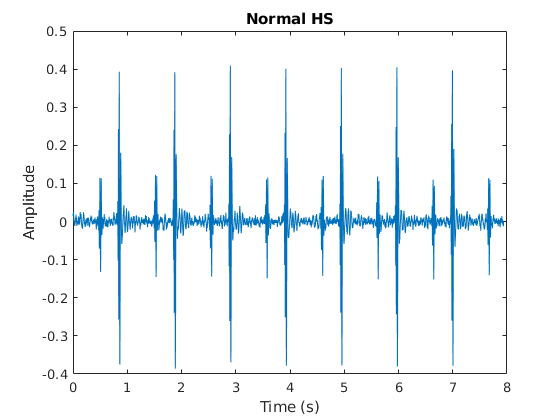
\includegraphics[scale = 0.45]{./normal.png}
    \caption{PCG of a Normal HS}
    \label{fig:normal}
\end{figure}{}

\subsection*{The Murmur Class}
The Murmur class consists of pathological HSs. Murmurs are produced when there is a turbulent blood flow between either systolic or diastolic periods \cite{35}. The turbulence often cause a "whooshing" sound in between S1 and S2 or in between S2 and S1. The illustration above shows the \textit{"lub, dub"} of a Murmur HS over time \cite{bentley}.

\hspace{1cm}{\texttt{lub..***..dub......lub..***..dub.....}}

\hspace{3.5cm} or 

\hspace{1cm}{\texttt{lub...dub...***...lub...dub..***...}}

Figure \ref{fig:murmur} illustrates a typical PCG of a Murmur HS.
\begin{figure}[h!]
    \centering
    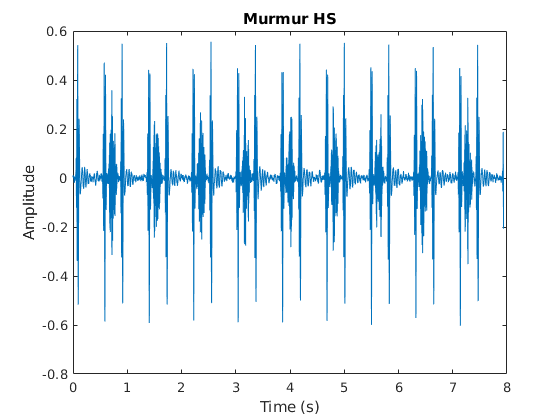
\includegraphics[scale = 0.45]{./murmur.png}
    \caption{PCG of a Murmur HS}
    \label{fig:murmur}
\end{figure}{}

From figure \ref{fig:murmur} it can clearly be seen that there are are extra disturbances in between S1 and S2 as compared to figure \ref{fig:normal}.

\subsection*{The Extra HS Class}
\label{sec:extra}
The Extra HS class does not necessarily consists of pathological HSs, however sometimes it could be a sign of a disease. Extra HS are produced when there is either an extra S2 or S1 after either S2 or S1 has occurred. This repeats regularly throughout the entire heart cycle in this manner S1-S2-S2-S1 or S1-S1-S2-S1-S1.
The illustration above shows the \textit{"lub, dub"} of a Extra HS over time \cite{bentley}.

\hspace{1cm}{\texttt{lub.lub...dub......lub.lub...dub.....}}

\hspace{3.5cm} or 

\hspace{1cm}{\texttt{lub...dub.dub.....lub...dub.dub.....}}

Figure \ref{fig:extra} illustrates a typical PCG of an Extra HS.
\begin{figure}[h!]
    \centering
    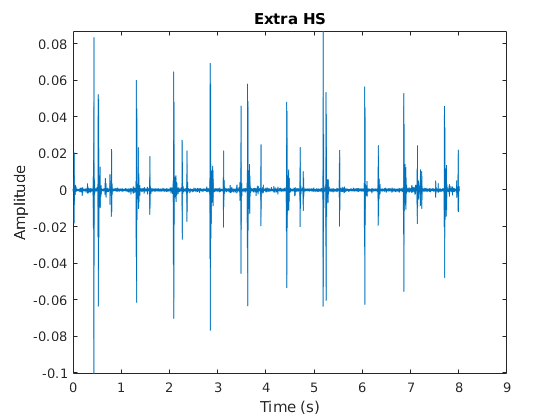
\includegraphics[scale = 0.45]{./extra.png}
    \caption{PCG of an Extra HS}
    \label{fig:extra}
\end{figure}{}

From figure \ref{fig:extra} it can clearly be seen that there are extra peak in between S1 and S2 as compared to figure \ref{fig:normal}.

\subsection*{The Extrasystole HS Class}
The Extrasystole class, similar to the \hyperref[sec:extra]{Extra HS} class, does not necessarily consists of pathological HSs, however sometimes it could be a sign of a disease. Extrasystole HSs occur in a similar manner as Extra HS, but they do not occur regularly. They are commonly identified by HSs that are out of place, with a HS either repeated or skipped. The illustration above shows the \textit{"lub, dub"} of a Extrasystole HS over time \cite{bentley}.

\hspace{0.5cm}{\texttt{lub....dub......lub.lub...dub.....lub....}}

\hspace{3.5cm} or 

\hspace{0.5cm}{\texttt{lub....dub.dub.....lub...dub......lub....}}

Figure \ref{fig:extrasys} illustrates a typical PCG of an Extrasystole HS.
\begin{figure}[h!]
    \centering
    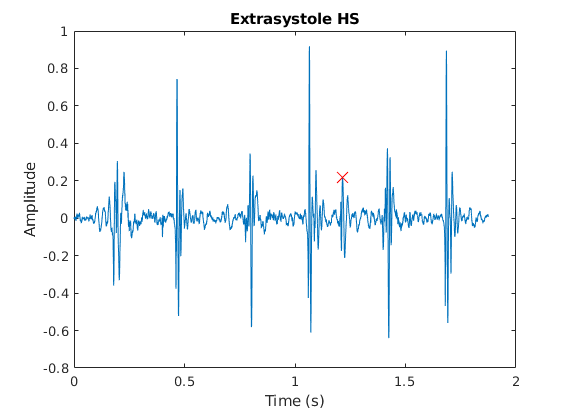
\includegraphics[scale = 0.45]{./extrasys.png}
    \caption{PCG of an Extrasystole HS}
    \label{fig:extrasys}
\end{figure}{}

From figure \ref{fig:extrasys} it can clearly be seen that there is a single extra peak in between S1 and S2, marked with a red cross, as compared to figure \ref{fig:normal} and figure \ref{fig:extra}.

\subsection*{The Artifact Class}
\label{sec:arti}
The Artifact class does not consist of any HSs. These are recordings of random sounds. The class is to help the developed models to differentiate between a HS and just pure noise \cite{bentley}.

Figure \ref{fig:arti} illustrates a typical of an Artifact.
\begin{figure}[h!]
    \centering
    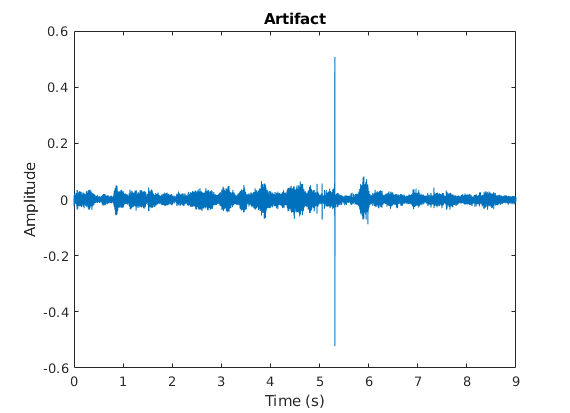
\includegraphics[scale = 0.45]{./arti.png}
    \caption{Artifact Class signal}
    \label{fig:arti}
\end{figure}{}

From figure \ref{fig:arti}, it can be seen that there is no sense of normal periodicity within the signal.

\section{Preprocessing \& Segmentation Phase}
\label{app:preseg}
Figure \ref{fig:preseg} presents the steps and processes taken in the preprocessing and segmentation phase. For a more clearer and concise explanation of the figure refer to \cite{love}.
%\vspace{-2cm}
\begin{figure}[h!]
    \centering
    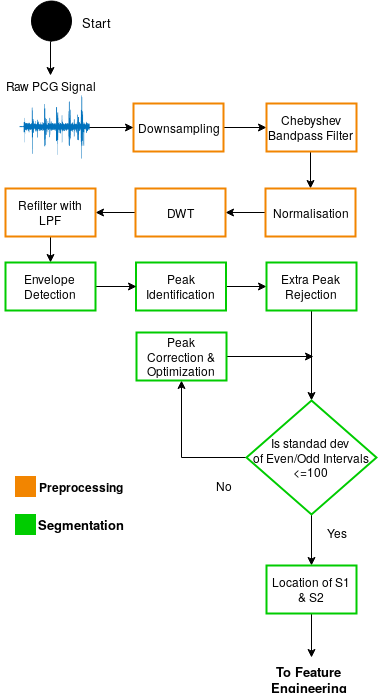
\includegraphics[scale=0.45]{./reportFDfinal.png}
    \caption{Preprocessing and Segmentation flow diagram}
    \label{fig:preseg}
\end{figure}{}

\section{Feature Extraction}
\label{app:features}
\subsection{Time Domain Features}
Table \ref{tab:tfeat} presents an elaboration of the different features extracted from the results of segmentation. Time-domain features make up the majority of the features with 10 out of 24 features coming from the this domain.

\begin{table}[h!]
\caption{Features from the time-domain}
\label{tab:tfeat}
\begin{tabular}{|l|l|}
\hline
\multicolumn{1}{|c|}{\textbf{Feature}} & \multicolumn{1}{c|}{\textbf{Description}} \\ \hline
\multicolumn{1}{|c|}{stdS1} & \multicolumn{1}{c|}{\label{t:s1}Standard deviation of systolic period.} \\ \hline
\multicolumn{1}{|c|}{stdS2} & \multicolumn{1}{c|}{\label{t:s2}Standard deviation of diastolic period.} \\ \hline
meanS1 & Mean of systolic period. \\ \hline
meanS2 & Mean of diastolic period. \\ \hline
maxstdS1 & \begin{tabular}[c]{@{}l@{}}Standard deviation of systolic period \\ after dropping the largest interval.\end{tabular} \\ \hline
maxstdS2 & \begin{tabular}[c]{@{}l@{}}Standard deviation of diastolic period \\ after dropping the largest interval.\end{tabular} \\ \hline
mmstdS1 & \begin{tabular}[c]{@{}l@{}}Standard deviation of systolic period \\ after dropping the largest and smallest\\ intervals.\end{tabular} \\ \hline
mmstdS2 & \begin{tabular}[c]{@{}l@{}}Standard deviation of diastolic period \\ after dropping the largest and smallest\\ intervals.\end{tabular} \\ \hline
prRatio & \begin{tabular}[c]{@{}l@{}}\label{t:pr}Ratio of the total number of peaks left\\ after Peak Rejection \cite{love} over\\ the length of the audio file\end{tabular} \\ \hline
pcRatio & \begin{tabular}[c]{@{}l@{}}\label{t:pc}Ratio of the total number of peaks left\\ after Peak Correction \cite{love} over \\ peaks from Peak Rejection.\end{tabular} \\ \hline
\end{tabular}
\end{table}

\subsection{Wavelet Features}
Table \ref{tab:wav} presents an elaboration of the different features extracted from DWT and wavelet denoising. Wavelet features make up the minority of the features with 3 out of 24 features coming from the this domain.

\begin{table}[h!]
\caption{Features extracted from DWT}
\label{tab:wav}
\begin{tabular}{|c|l|}
\hline
\textbf{Feature} & \multicolumn{1}{c|}{\textbf{Description}} \\ \hline
rebuildError & \begin{tabular}[c]{@{}l@{}}Average difference between the PCG\\ signal before denoising and the PCG\\ signal after denoising.\end{tabular} \\ \hline
stdWavelet & \begin{tabular}[c]{@{}l@{}}Standard deviation of the approxim-\\ ation of a  $6^{th}$ level db6 DWT \\ \\ of the preprocessed PCG signals.\end{tabular} \\ \hline
\multicolumn{1}{|l|}{meanWavelet} & \begin{tabular}[c]{@{}l@{}}Mean of the approximation of a $6^{th}$\\ level db6 DWT of the preprocessed\\ PCG signals.\end{tabular} \\ \hline
\end{tabular}
\end{table}

\subsection{Frequency Domain Features}

\subsubsection{Computation of the FFTSHA}
\label{sec:fftsha}
\textcolor{white}{Ke yaka degree ye!}\\
The below steps explain in details on how the FFTSHA of a PCG signal is computed. Figure \ref{fig:fftsha} illustrates the flow diagram of the computation. All the computation are done in MATLAB.

\begin{figure}[h!]
    \centering
    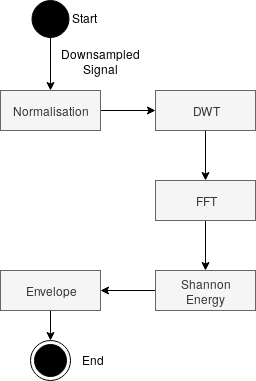
\includegraphics[scale=0.6]{./fftsha.png}
    \caption{Steps followed in computing FFTSHA}
    \label{fig:fftsha}
\end{figure}{}

Figure \ref{fig:fftsha} steps are explained in detail below.
\begin{enumerate}
    \item Downsample the PCG signal \& then normalise.
    \item Denoise the normalised and downsampled signal using $5^{th}$ level db7 DWT.
    \item Take the FFT of the denoised PCG signal.
    \item Compute the the Shannon Energy of the calculated FFT.
    \item Calculate the the envelope of the computed Shannon Energy using the 'analytic' option in MATLAB to get the FFTSHA.
\end{enumerate}{}

Figure \ref{fig:fftvsha} illustrates the differences between FFT and FFTSHA of a PCG signal.
\begin{figure}[h!]
    \centering
    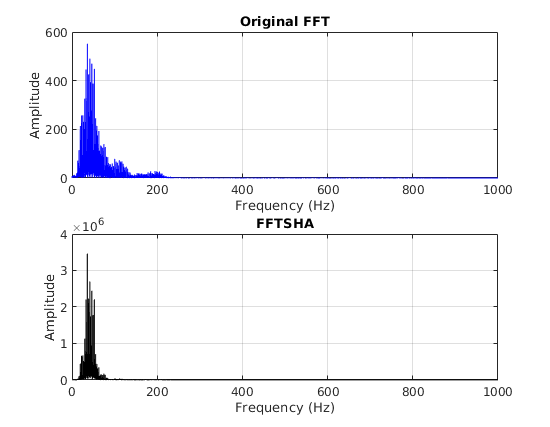
\includegraphics[scale=0.6]{./fftshavFFT.png}
    \caption{FFT vs FFTSHA of a PCG signal}
    \label{fig:fftvsha}
\end{figure}{}

From figure \ref{fig:fftvsha}  it can be seen that the FFTSHA appears to be a greatly attenuated version of the FFT. This characteristic is useful in the features extracted from the FFTSHA.

\subsubsection{Extracted Features}
\textcolor{white}{Ke yaka degree ye!}\\
Table \ref{tab:freq} presents an elaboration of the different features extracted from the frequency-domain. There a 5 features out of 24 that are extracted from this domain.
\begin{table}[h!]
\caption{Features extracted from the frequency-domain.}
\label{tab:freq}
\begin{tabular}{|l|l|}
\hline
\multicolumn{1}{|c|}{\textbf{Feature}} & \multicolumn{1}{c|}{\textbf{Description}} \\ \hline
\multicolumn{1}{|c|}{stdFFTSHA} & \begin{tabular}[c]{@{}l@{}}Standard deviation of the identified\\peaks in the {[}180 190{]} Hz band.\end{tabular} \\ \hline
\multicolumn{1}{|c|}{lenFFTSHA} & \begin{tabular}[c]{@{}l@{}}Count of qualifying peaks identified in\\ the {[}180 190{]} Hz band.\end{tabular} \\ \hline
stdlenFFTSHA & Ratio of stdFFTSHA over lenFFTSHA \\ \hline
lenstdFFTSHA & Ratio of lenFFTSHA over stdFFTSHA \\ \hline
posFFT & \begin{tabular}[c]{@{}l@{}}Count of peaks from Shannon Energy\\ of FFT.\end{tabular} \\ \hline
\end{tabular}
\end{table}

\subsection{Cepstrum Features}
Table \ref{tab:cep} presents an elaboration of the different features extracted from taking the PCA of MFCC coefficient vectors. Cepstrum features make up 6 out of the 24 features extracted.

\begin{table}[h!]

\caption{Features extracted from the cepstrum-domain.}
\label{tab:cep}

\begin{tabular}{|c|l|}
\hline
\textbf{Feature} & \multicolumn{1}{c|}{\textbf{Description}} \\ \hline
stdPCA1 & \begin{tabular}[c]{@{}l@{}}Standard deviation of the first \\ \\ PCA vector.\end{tabular} \\ \hline
meanPCA1 & Mean of the first PCA vector. \\ \hline
stdPCA2 & \begin{tabular}[c]{@{}l@{}}Standard deviation of the second\\ PCA vector.\end{tabular} \\ \hline
meanPCA2 & Mean of the second PCA vector. \\ \hline
\multicolumn{1}{|l|}{stdPCA3} & \begin{tabular}[c]{@{}l@{}}Standard deviation of the third\\ PCA vector.\end{tabular} \\ \hline
\multicolumn{1}{|l|}{meanPCA3} & Mean of the third PCA vector. \\ \hline
\end{tabular}
\end{table}

\section{Results}
\label{app:res}

Figure \ref{fig:anna} and Figure \ref{fig:annb} present the testing and training accuracy of ANN for Dataset A and Dataset B respectively.

\begin{figure}[h!]
    \centering
    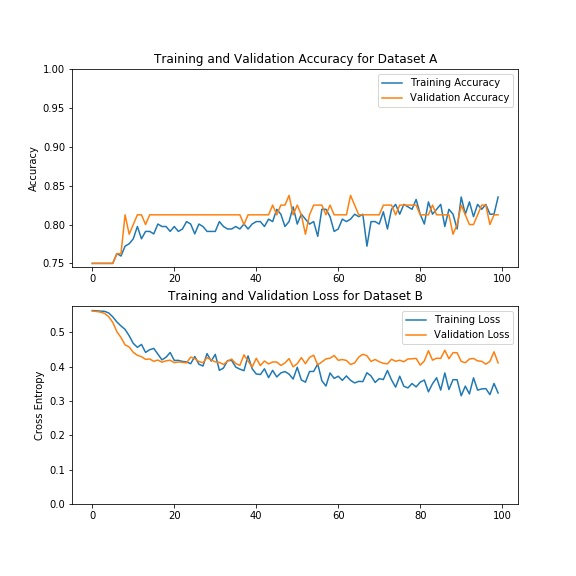
\includegraphics[scale=0.4]{./ANN_A.jpg}
    \caption{Training vs testing accuracy for Dataset B}
    \label{fig:anna}
\end{figure}{}

\newpage
.
\vspace{8.45cm}

\begin{figure}[h!]
    \centering
    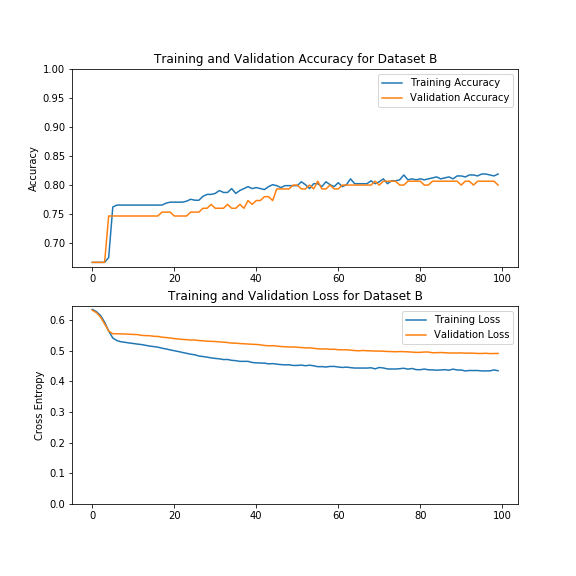
\includegraphics[scale=0.4]{./B_80_81_No_Dropout_Validation_split.png}
    \caption{Training vs testing accuracy for Dataset B}
    \label{fig:annb}
\end{figure}{}

The above matrix presents the confusion matrix for ANN on Dataset B. 
\[
 CM :
  \begin{bmatrix}
  \label{cm}
     E & M & N \\
     2 & 0 & 6  & E\\
     4 & 9 & 2 & M \\
     7 & 1 & 32 & N
  \end{bmatrix}
\]

\newpage
\onecolumn
%%%%%%%%%%%%%%MEETINGS CLEARANCE%%%%%%%%%%%%%%%%%%%%%%
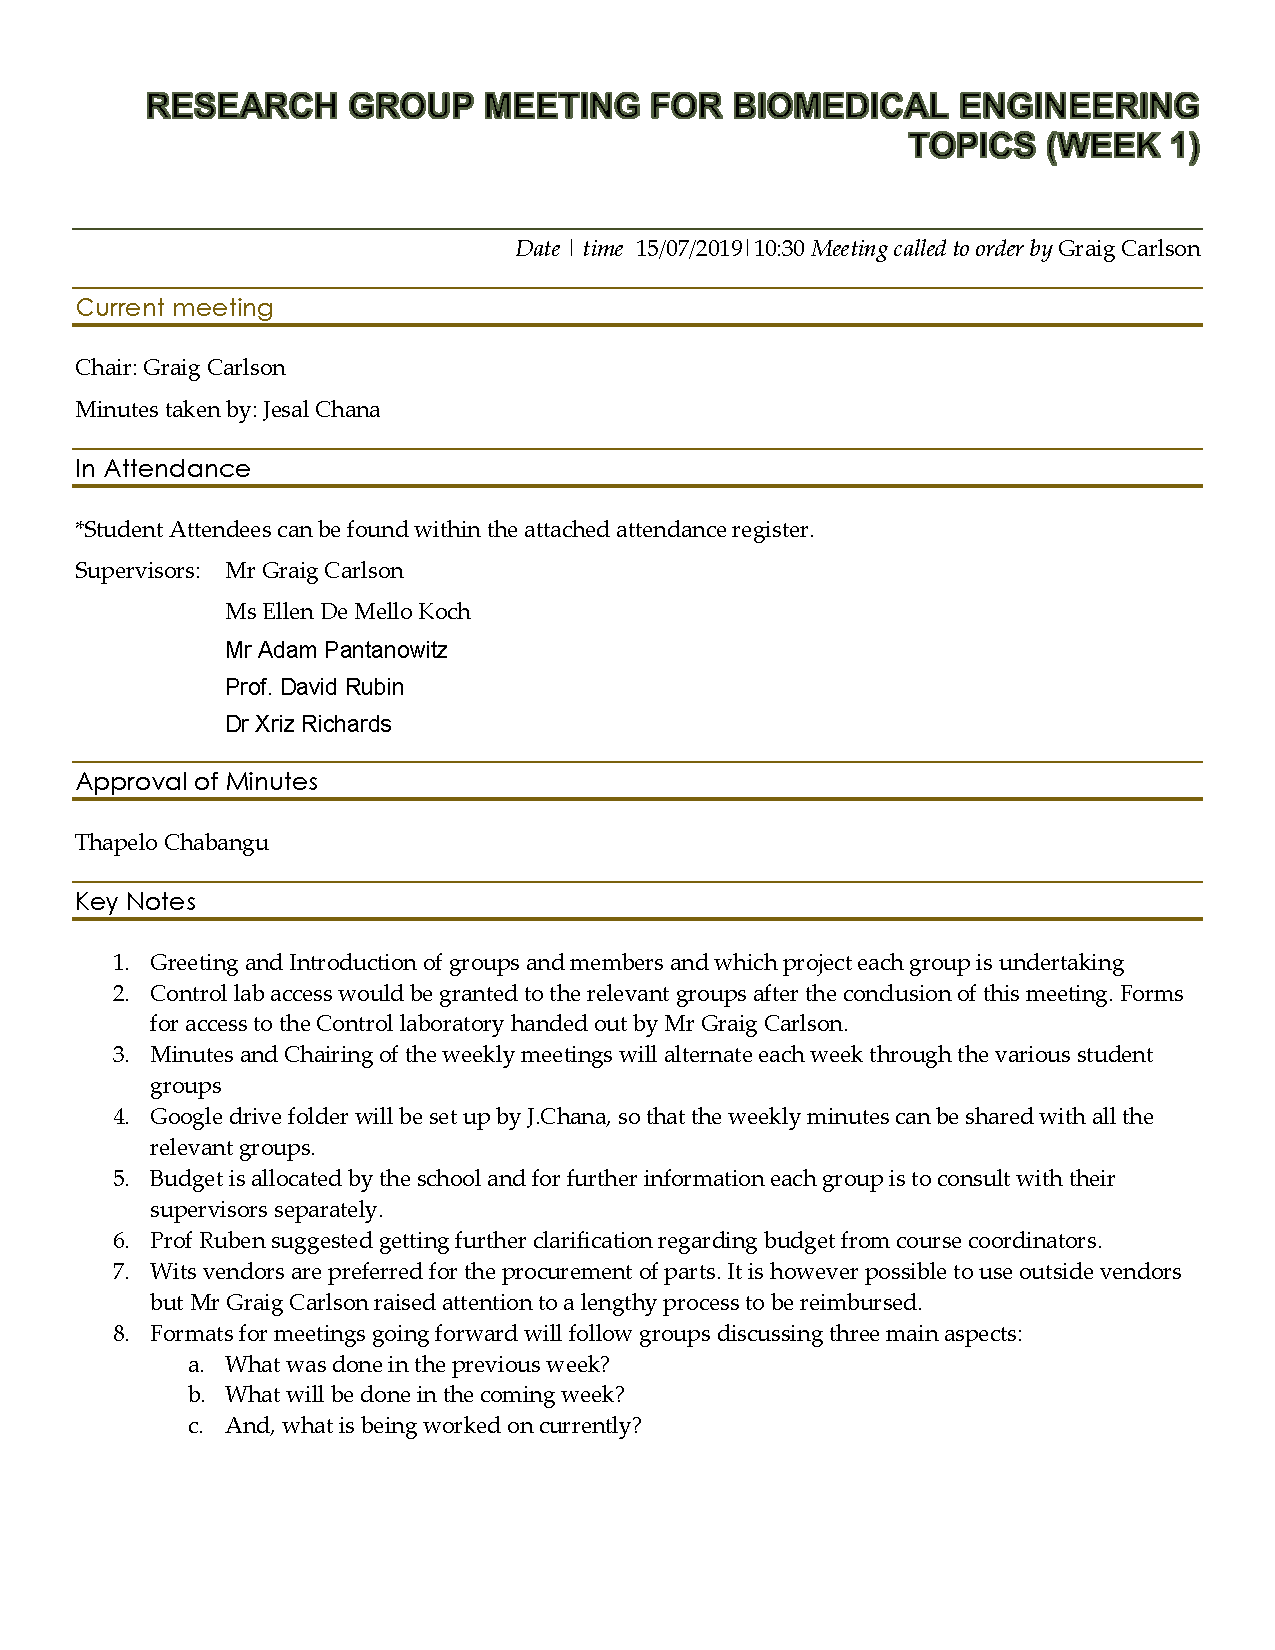
\includepdf[scale=0.94,pages=1,pagecommand={\section{MEETINGS MINUTES}\thispagestyle{empty}},fitpaper=true]{minutes.pdf}
\includepdf[scale=0.94,pages=2-32,pagecommand={\thispagestyle{empty}},fitpaper=true]{minutes.pdf}


\end{document}

" vim: ts=4
" vim: tw=78
" vim: autoindent
" vim: shiftwidth=4
